\documentclass[12pt,a4paper]{report}

% --- Paquets bàsics ---
\usepackage[catalan]{babel}
\usepackage[utf8]{inputenc}
\usepackage[T1]{fontenc}
\usepackage{lmodern}
\usepackage{geometry}
\usepackage{setspace}
\usepackage{graphicx}
\usepackage[hidelinks]{hyperref}
\usepackage{amsmath}
\usepackage{amsfonts}
\usepackage{amssymb}
\usepackage{float}
\usepackage{listings}
\usepackage{xcolor}

\lstdefinelanguage{CSharp}{
  language=[Sharp]C
}

\lstset{
  basicstyle=\ttfamily\footnotesize,
  breaklines=true,
  breakatwhitespace=false,
  postbreak=\mbox{\textcolor{red}{$\hookrightarrow$}\space},
  captionpos=b,
  frame=single,
  framerule=0.5pt,
  rulecolor=\color{gray!60},
  aboveskip=6pt,
  belowskip=6pt,
  keywordstyle=\color{blue},
  commentstyle=\color{gray},
  stringstyle=\color{teal},
  showstringspaces=false,
  tabsize=2
}
\begin{document}

\chapter{FONAMENTS TEÒRICS DE UNITY}

\section{Introducció a Unity}

\subsection{Què és Unity i per a què serveix}

La plataforma Unity (també coneguda com \textit{Unity3D} \ref{fig:logo_unity}) és un motor de desenvolupament en temps real utilitzat principalment per a la creació d'aplicacions interactives en 2D i 3D, especialment en l'àmbit dels videojocs. Aquest motor permet als desenvolupadors dissenyar, simular i executar entorns virtuals mitjançant una combinació d'un editor visual i un sistema de programació basat en \textit{scripts} \cite{Unity, lidon2025unity}.

A diferència d'altres eines més específiques, Unity es caracteritza per ser una plataforma multiplataforma, la qual permet desenvolupar una aplicació una sola vegada i exportar-la a diferents sistemes com ordinadors, dispositius mòbils, consoles o entorns web.

A nivell funcional, Unity proporciona eines per gestionar gràfics, física, il·luminació, animacions i interacció amb l'usuari, tot integrat dins d'un mateix entorn de desenvolupament \cite{UnityOfficial, UnityDocsManual}. Això facilita el procés de creació de projectes complexos sense necessitat de desenvolupar un motor des de zero.

\begin{figure}[H]
    \centering
    
\includegraphics[width=0.35\linewidth]{images/logo_unity.png}
    \caption{Logotip oficial del motor Unity}
    \label{fig:logo_unity}
\end{figure}

\subsection{Contextos d'aplicació de Unity}

Tot i que Unity va ser concebut inicialment com un motor per al desenvolupament de videojocs \cite{UnityWikipedia}, amb el pas del temps s'ha convertit en una eina utilitzada en múltiples àmbits gràcies a la seva flexibilitat i capacitat de simulació en temps real \cite{UnityLearnIntro}.

Actualment, Unity s'utilitza en sectors com:

\begin{itemize}
\item \textbf{Videojocs:} és un dels motors més utilitzats per desenvolupadors independents i estudis professionals.
\item \textbf{Simulació industrial:} permet crear bessons digitals i entorns virtuals per simular processos reals.
\item \textbf{Realitat virtual (VR) i realitat augmentada (AR):} facilita el desenvolupament d'experiències immersives.
\item \textbf{Arquitectura i enginyeria:} per visualitzar projectes en 3D abans de la seva construcció.
\item \textbf{Educació i recerca:} s'utilitza per crear entorns interactius i simulacions experimentals.
\end{itemize}

Aquesta versatilitat es deu al fet que Unity ha evolucionat d'un simple motor de videojocs a una plataforma general de creació de contingut interactiu en temps real.



\subsection{Evolució del motor Unity al llarg dels anys}

Unity va ser desenvolupat per l'empresa Unity Technologies i presentat per primera vegada l'any 2005. Inicialment, el seu objectiu era proporcionar un motor assequible per a desenvolupadors independents, que fins aquell moment tenien dificultats per accedir a tecnologies similars.

Amb el temps, Unity ha anat evolucionant tant en funcionalitats com en àmbits d'aplicació \cite{UnityLearnIntro}. En els seus inicis estava centrat exclusivament en el desenvolupament de videojocs, però progressivament ha incorporat millores en el renderitzat, la física, la compatibilitat multiplataforma i la integració amb noves tecnologies com la realitat virtual o la intel·ligència artificial.

Un dels aspectes més rellevants de la seva evolució és la seva contribució a la democratització del desenvolupament, permetent que usuaris amb pocs recursos puguin crear aplicacions complexes sense necessitat de desenvolupar eines pròpies.

Actualment, Unity és considerat un dels motors de desenvolupament més utilitzats a nivell mundial, amb una gran comunitat d'usuaris i una àmplia documentació disponible \cite{UnityWikipedia}.

\section{Característiques generals del motor}

\subsection{Treball en entorns 2D i 3D}

Unity permet desenvolupar aplicacions tant en 2D com en 3D dins d'un mateix entorn de treball.

En entorns 2D, proporciona eines específiques com el sistema de \textit{Sprites}, física 2D independent i càmeres ortogràfiques, facilitant el desenvolupament d'aplicacions basades en gràfics plans.

En entorns 3D, incorpora un sistema complet de representació espacial amb càmeres en perspectiva, il·luminació avançada i simulació física tridimensional, permetent desenvolupar entorns immersius com el bessó digital d'aquest projecte \cite{Unity2Dor3D}.

\subsection{Capacitats de renderització}

Unity disposa d'un sistema de renderització en temps real basat en la GPU, que permet visualitzar escenes de forma eficient \cite{GPUWikipedia}. 

Ofereix diferents \textit{Render Pipelines} \cite{UnityRenderPipelines}, entre els quals destaquen:
\begin{itemize}
    \item \textbf{Built-in Render Pipeline}: sistema clàssic amb configuració senzilla però menys flexible.
    \item \textbf{Universal Render Pipeline (URP)}: utilitzat en aquest projecte per oferir un bon equilibri entre rendiment i qualitat.
    \item \textbf{High Definition Render Pipeline (HDRP)}: orientat a visualitzacions d'alt realisme.
\end{itemize}

Aquesta flexibilitat permet adaptar el motor a diferents necessitats, des de simulacions senzilles fins a entorns visuals complexos.


%\begin{center}
%\url{https://en.wikipedia.org/wiki/Graphics_processing_unit}
%\end{center}
%

\subsection{Tipus de projectes que es poden desenvolupar}

Unity permet crear diferents tipus de projectes segons la configuració inicial seleccionada dins del \textit{Unity Hub} \ref{fig:menu_unity}. Entre els principals tipus destaquen \cite{UnityProjectTemplates}:

\begin{itemize}
    \item \textbf{Projectes 2D}: orientats a videojocs o aplicacions amb gràfics plans.
    \item \textbf{Projectes 3D (URP)}: utilitzats en la majoria d'aplicacions, incloent simulacions industrials com la desenvolupada en aquest treball.
    \item \textbf{Projectes HDRP}: enfocats a visualitzacions d'alt realisme (arquitectura, simulació avançada).
    \item \textbf{Realitat Virtual (VR)}: per al desenvolupament d'entorns immersius amb dispositius com ulleres VR.
    \item \textbf{Realitat Augmentada (AR)}: aplicacions que combinen elements virtuals amb el món real.
    \item \textbf{Mixed Reality (MR)}: combinació avançada de VR i AR.
\end{itemize}


\begin{figure}[H]
    \centering
    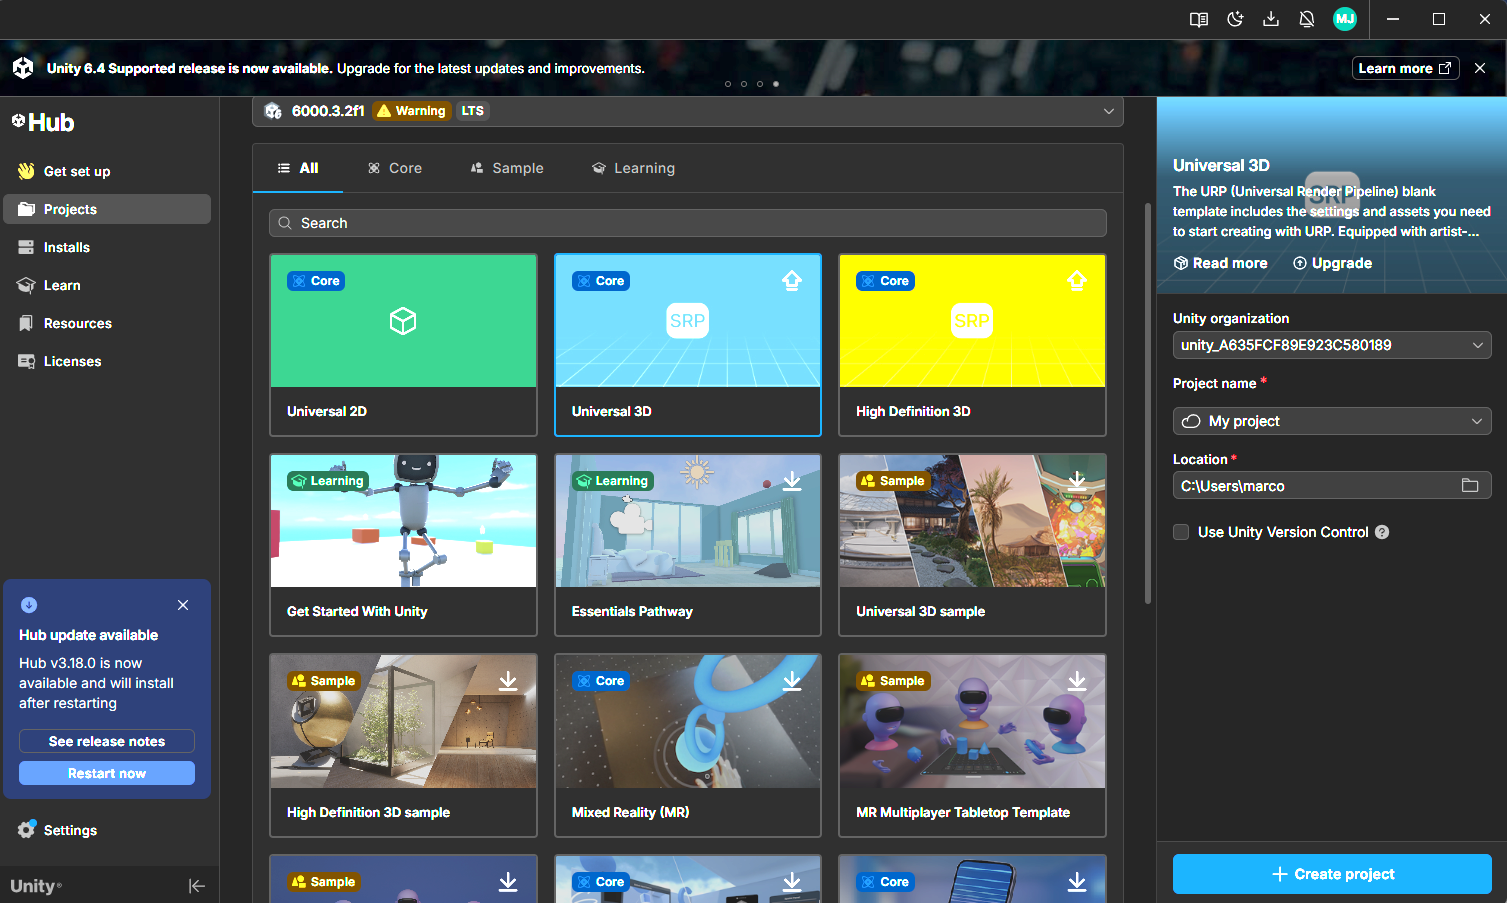
\includegraphics[width=0.35\linewidth]{images/menu_unity_1.png}
    \caption{Menu de projectes}
    \label{fig:menu_unity}
\end{figure}

\subsection{Procés de creació d'un projecte}

La creació d'un projecte a Unity segueix una sèrie de fases que permeten desenvolupar aplicacions de manera estructurada i modular. Inicialment, des del \textit{Unity Hub} es crea un nou projecte seleccionant la plantilla més adequada segons el tipus d'aplicació que es vol desenvolupar \cite{UnityCreateProject}.

Una vegada creat el projecte, el desenvolupament es basa principalment en la construcció d'escenes (\textit{Scenes}), que representen els diferents espais o entorns de treball dins de l'aplicació \cite{UnityScenes}. A partir d'aquí, el procés habitual de desenvolupament inclou les següents etapes:

\begin{itemize}
    \item Creació de l'escena i col·locació dels objectes
    \item Importació de models 3D, materials i textures
    \item Configuració de components i propietats físiques
    \item Programació del comportament mitjançant scripts en C\#
    \item Execució, simulació i proves del sistema
\end{itemize}

Aquest procés de treball permet desenvolupar aplicacions de forma iterativa, facilitant la modificació i ampliació del projecte durant totes les fases del desenvolupament. En aquest treball, aquesta metodologia ha permès construir la simulació de la planta industrial de manera modular i escalable.
\section{Entorn de desenvolupament de Unity}

\subsection{Estructura general de l'editor}

L'editor de \textit{Unity} \cite{UnityEditorInterface} està format per diferents finestres que permeten gestionar tots els elements d'un projecte de manera visual i interactiva. Aquest entorn es pot personalitzar segons les necessitats de l'usuari, però per defecte presenta una distribució estàndard amb les principals eines de desenvolupament.

Com es mostra a la figura \ref{fig:MenuEditor} són la vista d'escena (\textit{Scene}), la vista de joc (\textit{Game}), la jerarquia (\textit{Hierarchy}), l'inspector (\textit{Inspector}), la consola (\textit{Console}) i la finestra de projecte (\textit{Project}).

\begin{figure}[H]
    \centering
    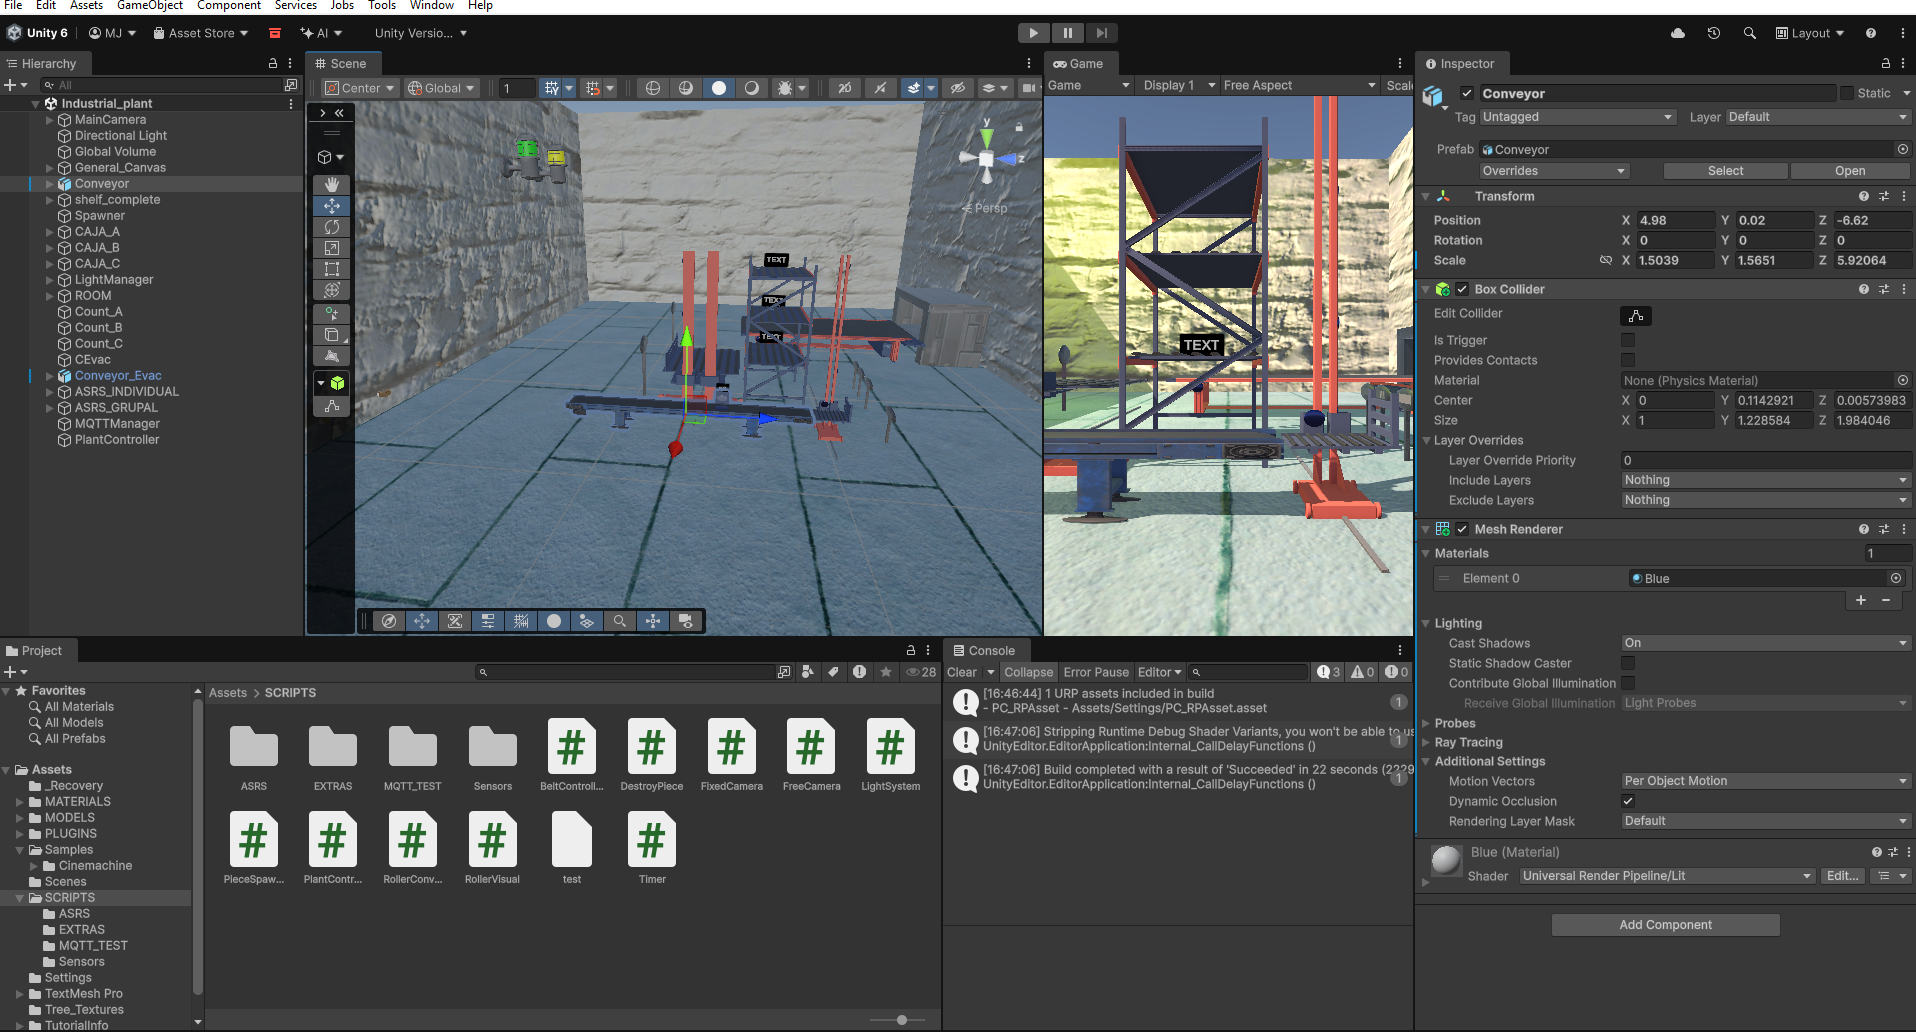
\includegraphics[width=0.95\linewidth]{images/menu_editor.png}
    \caption{Interfície general de l'editor de Unity amb les principals finestres de treball}
    \label{fig:MenuEditor}
\end{figure}


\subsection{Vista Scene}

La vista \textit{Scene} \cite{UnityScenes} és l'espai on es construeix el món virtual. Permet visualitzar i manipular els objectes en un entorn 2D o 3D, modificar la seva posició, rotació i escala, així com organitzar-los dins de l'escena. Aquesta vista és \textbf{interactiva} i no representa el resultat final del joc, sinó una eina de disseny.



\subsection{Vista Game}

La vista \textit{Game} mostra la representació final del joc tal com la veuria l'usuari. Aquesta vista depèn de les càmeres de l'escena i permet executar el projecte en temps real mitjançant el botó de \textit{Play}.



\subsection{Inspector}

L'\textit{Inspector} \cite{UnityInspector} és una de les eines més importants de Unity, ja que permet visualitzar i modificar totes les propietats dels objectes seleccionats. Quan es selecciona un objecte, l'Inspector mostra tots els seus components (transformacions, materials, scripts, etc.) i permet editar-los (figura \ref{fig:menu_editor_inspector}).

\begin{figure}[H]
    \centering
    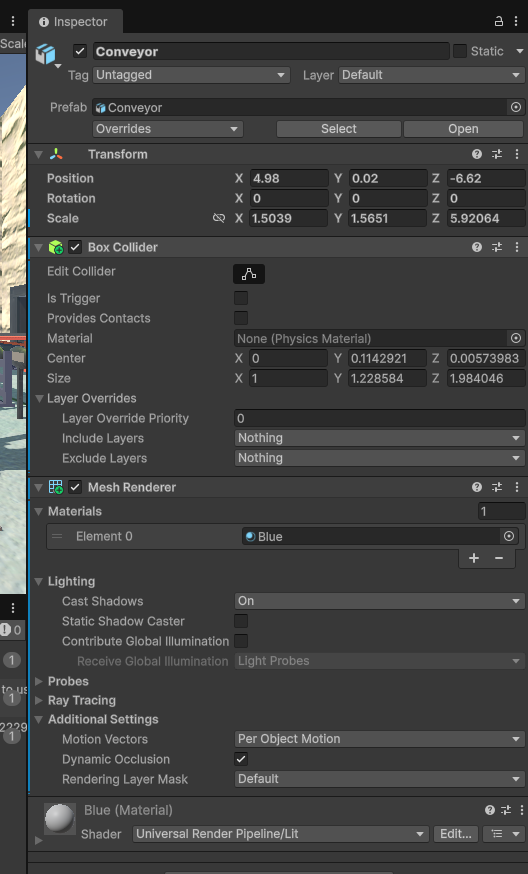
\includegraphics[width=0.3\linewidth]{images/menu_editor_insp.png}
    \caption{Finestra Inspector de Unity amb les propietats i components d'un objecte seleccionat}
    \label{fig:menu_editor_inspector}
\end{figure}


\subsubsection{Gestió de components}

Cada objecte a Unity està format per components \cite{UnityComponents}. Aquests defineixen el seu comportament i característiques (per exemple, \textit{Transform}, \textit{Renderer}, \textit{Collider} o scripts personalitzats). Des de l'Inspector es poden afegir nous components mitjançant el botó \textit{Add Component}, així com modificar les seves propietats.

\subsubsection{Tags i Layers}

Unity permet assignar \textit{Tags} i \textit{Layers} als objectes per facilitar la seva identificació i gestió \cite{UnityTags2023}.

\begin{itemize}
    \item \textbf{Tags}: permeten identificar objectes (per exemple, "Player" o "Box").
    \item \textbf{Layers}: s'utilitzen principalment per controlar col·lisions i càmeres.
\end{itemize}


\subsubsection{Gestió de paquets (Package Manager)}

El \textit{Package Manager} \cite{UnityPackageManager} és una eina integrada en Unity que permet afegir i gestionar funcionalitats addicionals mitjançant paquets, els quals inclouen recursos, scripts i eines que amplien les capacitats del motor. \cite{UnityPackagesDocs} Aquesta eina facilita la instal·lació i actualització de components dins del projecte des d'una única interfície (figura \ref{fig:package_manager}). 
En aquest projecte s'han utilitzat alguns paquets rellevants:

\begin{itemize}

\item \textbf{Cinemachine}: Permet gestionar càmeres de forma avançada. Tot i que inicialment es va considerar per al control de càmera, finalment s'han reutilitzat alguns recursos visuals del paquet. \cite{UnityCinemachine}

\item \textbf{FBX Exporter}: Utilitzat per exportar models en format \textit{.fbx} i editar-los en eines externes (\textit{Blender}).

\item \textbf{Input System}: Sistema d'entrada de dades més flexible que permet gestionar diferents dispositius.

\item \textbf{ProBuilder}: Eina de modelatge integrada utilitzada per crear geometria directament dins de Unity.

\end{itemize}

\begin{figure}[h]
    \centering
    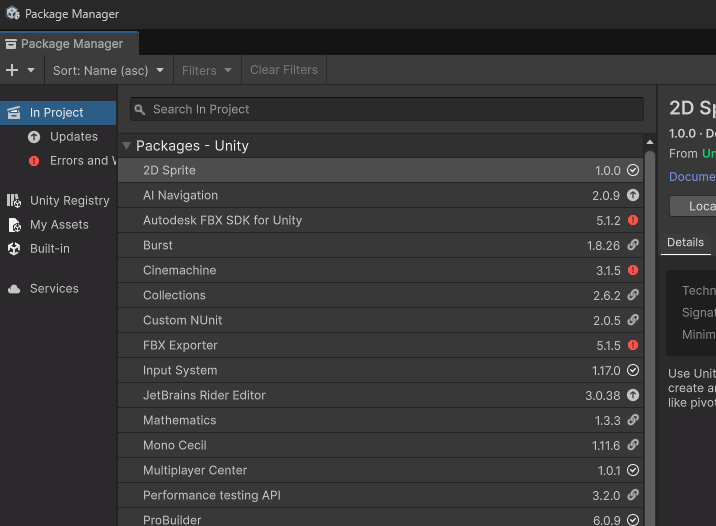
\includegraphics[width=0.5\linewidth]{images/unity_package_manager.png}
    \caption{Interfície del Package Manager de Unity per gestionar paquets i funcionalitats addicionals}
    \label{fig:package_manager}
\end{figure}


\subsection{Hierarchy}

La finestra \textit{Hierarchy} \cite{UnityHierarchy} mostra tots els objectes (\textit{GameObjects}) presents en l'escena actual, organitzats en forma d'arbre jeràrquic.

\begin{figure}[H]
    \centering
    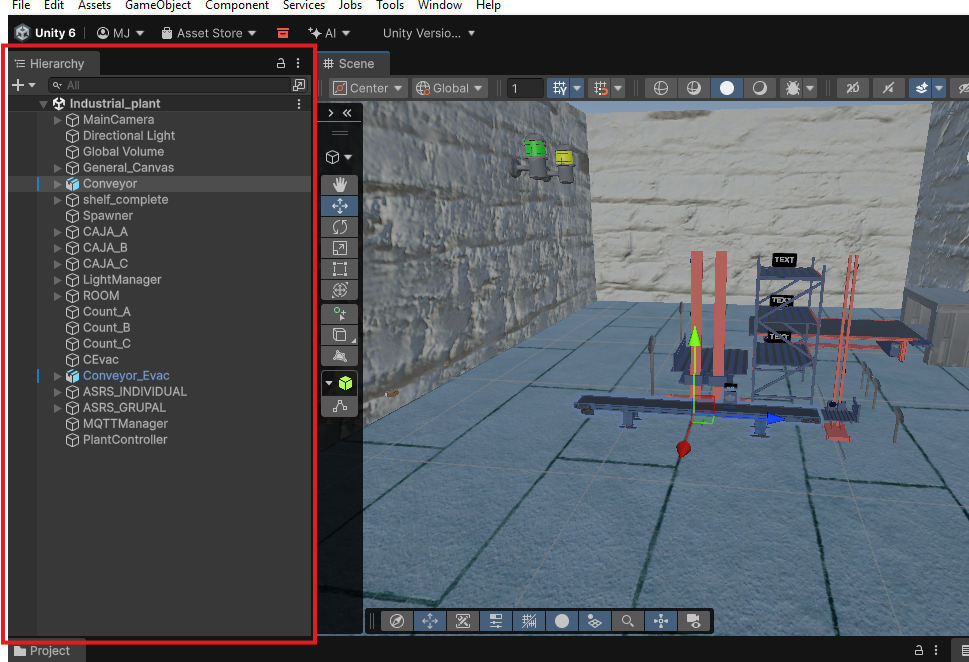
\includegraphics[width=0.6\linewidth]{images/menu_editor_hier.png}
    \caption{Finestra Hierarchy que mostra l'estructura jeràrquica dels GameObjects dins de l'escena}
\end{figure}

Aquesta estructura permet establir relacions pare-fill entre objectes, facilitant la seva organització i manipulació. 

\subsection{Console}

La consola (\textit{Console}) és l'eina que mostra missatges del sistema, errors i advertències generades durant l'execució del programa. És essencial per detectar errors en scripts i depurar el funcionament del sistema.

\subsection{Barra superior}

La barra superior de Unity conté els principals menús de gestió del projecte i accés a funcionalitats avançades del motor (figura \ref{fig:barra_superior}). 

\begin{figure}[H]
    \centering
    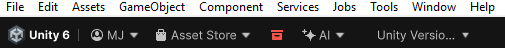
\includegraphics[width=0.6\linewidth]{images/barra_superior.png}
    \caption{Barra superior del menú editor en Unity}
    \label{fig:barra_superior}
\end{figure}

\begin{itemize}

\item \textbf{File}: permet crear, obrir i guardar projectes i escenes.

\item \textbf{Edit}: inclou opcions de configuració, preferències i eines d'edició generals.

\item \textbf{Assets}: gestiona els recursos del projecte, permetent importar, exportar i organitzar fitxers.

\item \textbf{GameObject}: permet crear nous objectes dins de l'escena, com càmeres, llums o objectes buits.

\item \textbf{Component}: s'utilitza per afegir components als objectes seleccionats, definint el seu comportament.

\item \textbf{Services}: dona accés a serveis externs de Unity com analítica, multiplayer o monetització.

\item \textbf{Jobs}: relacionat amb el sistema de processament paral·lel de Unity per optimitzar el rendiment.

\item \textbf{Tools}: inclou eines addicionals, tant pròpies com instal·lades mitjançant paquets.

\item \textbf{Window}: permet obrir i gestionar les diferents finestres de l'editor, incloent el \textit{Package Manager}.

\item \textbf{Help}: proporciona accés a la documentació oficial, tutorials i suport.

\end{itemize}

\section{Gestió de materials i textures}

\subsection{Idees bàsiques respecte als materials}

En Unity, un \textit{material} defineix l'aspecte visual d'un objecte dins de l'escena, incloent propietats com el color, la brillantor o la resposta a la llum. \cite{UnityMaterialsIntro}

Els materials es creen des del panell de \textit{Project} i es configuren a l'\textit{Inspector}. Cada material està associat a un \textbf{Shader}, que determina com es representa visualment l'objecte. \cite{UnityShaders}

Pel que fa a l'assignació d'aquests, els materials s'assignen als objectes mitjançant el component \textit{Mesh Renderer}, encarregat de la seva representació visual.

Aquesta assignació es pot fer directament des de l'\textit{Inspector} o arrossegant el material sobre l'objecte. Un mateix material pot ser compartit entre diversos objectes. \cite{UnityMaterialReference}


\subsection{Importació de textures externes}

Les textures són imatges que aporten detall visual als materials, com el color o el relleu. \cite{UnityMaterialsIntro}

En aquest projecte s'han utilitzat textures PBR (\textit{Physically Based Rendering}) provinents de repositoris externs, que permeten aconseguir resultats més realistes.

El procés bàsic d'ús és:

\begin{enumerate}

\item \textbf{Importació de les textures}: Les textures s'afegeixen al projecte arrossegant-les a la carpeta \textit{Assets}. \cite{UnityImportTextures}


\item \textbf{Creació del material}: Es crea un material que actuarà com a contenidor de les textures.

\item \textbf{Assignació de mapes PBR}: Les textures s'assignen als canals corresponents del material, com el color base o el relleu (normal map), per definir el seu comportament visual.

\begin{itemize}

\item \textbf{Albedo (Base Map)}: color base del material.

\item \textbf{Normal Map}: detall superficial (relleu).  
\item \textbf{Metallic Map}:parts metàl·liques del material (actuació davant la llums)

\item \textbf{Height Map}: profunditat o desplaçament en la superfície del material.

\item \textbf{Ambient Occlusion (AO)}: ombres suaus on la llum arriba més difícilment

\end{itemize}


\item \textbf{Configuració del tipus de textura}: Algunes textures requereixen ajustos específics a l'\textit{Inspector}, com el cas dels \textit{Normal Maps}. \cite{UnityImportTextures}


\item \textbf{Ajust de propietats del material}: Després una vegada tens tots els elements seleccionats, sempre existeix la opció de modificar aquestes textures segons sembli més correcte a cadascú.

\end{enumerate}



\subsection{Propietats dels materials (shader, color, tiling, offset)}

Els materials disposen de diverses propietats bàsiques:

\begin{itemize}

\item \textbf{Shader}: defineix com el material interactua amb la llum. \cite{UnityShaders}


\item \textbf{Color}: estableix el color base del material.


\item \textbf{Color}: estableix el color base del material.


\item \textbf{Offset}: permet desplaçar la textura dins de l'objecte. \cite{UnityTextureProperties}


\end{itemize}

Aquestes propietats permeten ajustar i reutilitzar materials de forma eficient dins de l'escena.

Addicionalment, Unity utilitza tècniques com el \textit{Physically Based Rendering (PBR)} per aconseguir resultats realistes sota diferents condicions d'il·luminació. \cite{UnityMaterialsIntro}

\section{Sistema de components en Unity}

\subsection{Concepte de GameObject}

En Unity, qualsevol element dins d'una escena es representa mitjançant un \textit{GameObject}, que actua com la unitat bàsica del sistema. Aquest pot representar tant objectes visibles com elements lògics. Un \textit{GameObject} no té funcionalitat per si sol; el seu comportament ve determinat pels components associats, seguint un model modular basat en composició. \cite{UnityGameObjects}


\subsection{Sistema de components}

Unity utilitza un sistema basat en components, on cada \textit{GameObject} pot contenir múltiples components que defineixen les seves propietats i comportament.

Aquest enfocament segueix el paradigma de \textit{composition over inheritance} \cite{UnityComponents}, molt utilitzat en el desenvolupament de videojocs, ja que permet reutilitzar funcionalitats de manera eficient.

Alguns exemples de components habituals són:

\begin{itemize}
\item \textbf{Transform}: defineix la posició, rotació i escala de l'objecte.
\item \textbf{Renderer}: permet visualitzar l'objecte.
\item \textbf{Collider}: defineix la seva forma física per a col·lisions.
\item \textbf{Rigidbody}: permet aplicar física realista.
\item \textbf{Scripts}: defineixen comportaments personalitzats.
\end{itemize}

Aquest sistema modular permet afegir o eliminar funcionalitats sense modificar l'estructura interna de l'objecte, facilitant el desenvolupament i manteniment del projecte.

\subsection{Component Rigidbody}

El \textit{Rigidbody} \cite{UnityRigidbody} permet aplicar física als objectes, com forces, gravetat i col·lisions, sent essencial en simulacions com el moviment de peces on es busca que hi hagi interacció de peces i que tingui un comportament relativament realista.


\subsubsection{Propietats principals}

El \textit{Rigidbody} disposa de diverses propietats que controlen el seu comportament:

\begin{itemize}
\item \textbf{Mass}: defineix la massa de l'objecte.
\item \textbf{Drag}: resistència al moviment lineal.
\item \textbf{Angular Drag}: resistència a la rotació.
\end{itemize}


\paragraph{Diferència entre \textit{isKinematic} i \textit{useGravity}}

Dins del component \textit{Rigidbody}, dues propietats especialment rellevants són \textit{isKinematic} i \textit{useGravity}, ja que determinen com l'objecte interactua amb el sistema de física de Unity.

\begin{itemize}

\item \textbf{useGravity}:  
Quan aquesta propietat està activada, l'objecte es veu afectat per la gravetat global definida al motor físic. Això implica que l'objecte caurà si no hi ha cap suport que el mantingui en posició.

\item \textbf{isKinematic}:  
Quan està activada, el \textit{Rigidbody} deixa de ser controlat pel motor físic. Això significa que no respon a forces ni a col·lisions físiques i que el moviment s'ha de controlar manualment mitjançant scripts.

\end{itemize}

Un \textit{Rigidbody} cinemàtic pot ser mogut per codi però no reacciona a forces ni col·lisions com un cos físic normal. \cite{UnityColliders}

En el context d'aquest projecte, aquesta diferenciació és especialment important. Per exemple, els objectes poden tenir la gravetat activada per comportar-se de manera realista sobre les cintes transportadores, mentre que altres elements com actuadors o parts del sistema es controlen manualment mitjançant scripts, utilitzant \textit{isKinematic}.


\subsubsection{Configuració de la física}

Unity utilitza el motor físic NVIDIA PhysX \cite{UnityPhysics} per gestionar les simulacions físiques, permetent calcular col·lisions, forces i moviments de manera eficient.


Els càlculs físics es realitzen principalment dins del mètode \texttt{FixedUpdate()}, que s'executa a intervals regulars, garantint estabilitat en la simulació.

\subsubsection{Restriccions i comportament}

El \textit{Rigidbody} permet restringir moviments en determinats eixos mitjançant les opcions de \textit{Constraints}, ajudant a que els moviments poguin ser controlats i previsibles.

Per exemple:

\begin{itemize}
\item Bloquejar la rotació en els eixos X i Z per evitar inestabilitat.
\item Limitar el moviment en un eix concret.
\end{itemize}


\subsection{Component Collider}

Els \textit{Colliders} \cite{UnityColliders} defineixen la forma física d'un objecte per a la detecció de col·lisions. No són visibles, però són essencials per a la interacció entre objectes.

\subsubsection{Tipus de colliders}

Unity ofereix diferents tipus de colliders segons la geometria:

\begin{itemize}
\item \textbf{Box Collider}: forma cúbica.
\item \textbf{Sphere Collider}: forma esfèrica.
\item \textbf{Capsule Collider}: forma cilíndrica amb extrems arrodonits.
\item \textbf{Mesh Collider}: adapta la forma exacta del model.
\end{itemize}

L'ús correcte del tipus de collider és important per equilibrar precisió i rendiment.

\subsubsection{Mode Trigger}

Poden funcionar en mode \textit{Trigger}, permetent detectar objectes sense col·lisió física, fet útil per simular sensors industrials. Aquest mode s'utilitza mitjançant esdeveniments com \texttt{OnTriggerEnter()}, \texttt{OnTriggerExit()} o \texttt{OnTriggerStay()}. Aquest tipus de detecció és molt útil en sistemes industrials per simular sensors.

\subsubsection{Detecció de col·lisions}

Quan dos objectes amb colliders interactuen, Unity pot generar esdeveniments de col·lisió com\texttt{OnCollisionEnter()}, \texttt{OnCollisionExit()} o \texttt{OnCollisionStay()}. Aquest sistema permet detectar impactes físics reals dins del motor.

\subsection{Component Renderer}

El component \textit{Renderer} \cite{UnityRenderer} és responsable de la representació visual dels objectes dins de l'escena. Aquest component permet mostrar un objecte utilitzant un model 3D i un material associat. Sense un \textit{Renderer}, l'objecte no és visible dins de la escena. El \textit{Renderer} utilitza materials per definir l'aparença visual de l'objecte. Aquests materials inclouen shaders i textures que determinen com interactua amb la llum.


\subsection{Component Light}

El component \textit{Light} \cite{UnityLighting} és l'encarregat de simular les fonts de llum dins de l'escena de Unity i determina com els objectes són il·luminats i com es perceben materials, textures i volums. Les llums influeixen directament en el procés de renderització, afectant el color, la intensitat i les ombres dels objectes dins de l'entorn virtual.

\subsubsection{Tipus de llums}

Unity ofereix diferents tipus de llums segons el seu comportament:

\begin{itemize}
\item \textbf{Directional Light}: Il·lumina tots els objectes en una mateixa direcció sense importar la seva posició (sol).

\item \textbf{Point Light}: Llum en totes les direccions des d'un punt concret, similar a una bombeta. La seva intensitat disminueix amb la distància.

\item \textbf{Spot Light}: Llum focalitzada en forma de con

\item \textbf{Area Light}:  
Utilitzada principalment en renderització avançada, simula una superfície emissora de llum.
\end{itemize}

\subsubsection{Propietats principals}

El component \textit{Light} disposa de diverses propietats configurables des de l'\textit{Inspector}:

\begin{itemize}
\item \textbf{Color}: defineix el color de la llum.
\item \textbf{Intensity}: controla la intensitat lumínica.
\item \textbf{Range}: determina l'abast de la llum (especialment en \textit{Point Light} i \textit{Spot Light}).
\item \textbf{Shadows}: permet activar o desactivar la generació d'ombres.
\end{itemize}


En el context d'aquest projecte, la il·luminació no només té una funció estètica, sinó també funcional. Per exemple, es poden utilitzar llums per indicar l'estat del sistema, com senyals lluminoses (verd, groc, vermell) similars a les utilitzades en entorns industrials reals. A més, la possibilitat d'activar o desactivar llums mitjançant scripts permet simular comportaments com alarmes o indicadors d'estat dins del bessó digital.


\section{Fonaments de programació en Unity}

\subsection{Introducció a la programació en Unity}

Unity permet implementar el comportament dels objectes mitjançant scripts, que defineixen la lògica del sistema. Aquests scripts s'associen als \textit{GameObjects} i s'executen automàticament segons el cicle de vida del motor.

El sistema de programació de Unity es basa en el concepte de components, on cada script actua com un comportament independent que es pot reutilitzar en diferents objectes.

\subsection{Llenguatge utilitzat i llibreries principals}

El llenguatge principal utilitzat en Unity és \textbf{C\#} \cite{UnityProgrammingGuide}, integrat amb la plataforma \textit{.NET}. Aquest llenguatge permet una programació orientada a objectes robusta i flexible.

Els scripts en Unity hereten habitualment de la classe \textit{MonoBehaviour}, que proporciona accés a les funcionalitats del motor com el sistema de física, el temps o la gestió d'objectes.

A més, s'utilitzen llibreries com:

\begin{itemize}
\item \texttt{UnityEngine}: proporciona accés a tots els components del motor (Transform, Rigidbody, etc.)
\item \texttt{System.Collections} \cite{dotnet_collections}: permet gestionar col·leccions de dades
\end{itemize}


\subsection{Estructura d'un script en Unity}

Els scripts en Unity segueixen un cicle de vida determinat, en el qual existeixen una sèrie de funcions que s'executen automàticament en funció de l'estat de l'objecte.

\subsubsection{Mètodes principals}

\begin{itemize}

\item \textbf{Awake}: Primer mètode que es crida i serveix per inicialitzar variables internes.

\item \textbf{Start}:  
S'executa abans del primer frame, després de \textit{Awake}.\cite{UnityExecutionOrder}

\item \textbf{Update}:  
S'executa una vegada per cada frame. És el mètode principal per a la lògica del joc i la gestió d'entrada.

\item \textbf{FixedUpdate}:  
S'executa a intervals de temps fixos i s'utilitza principalment per a càlculs físics.

\end{itemize}

\textit{FixedUpdate} s'ha d'utilitzar per treballar amb \textit{Rigidbody}, mentre que \textit{Update} s'utilitza per la lògica general. \cite{UnityUpdate}


\subsection{Gestió del temps}

Unity proporciona un sistema de control temporal \cite{UnityTime} per garantir que els moviments siguin independents del nombre de frames per segon.

\begin{enumerate}
    \item Time.deltaTime: Representa el temps transcorregut entre dos frames consecutius. S'utilitza per garantir que el moviment sigui constant independentment del rendiment del sistema.
    \item Time.fixedDeltaTime: Representa l'interval de temps fix utilitzat en \textit{FixedUpdate}, especialment en càlculs físics.

\textit{Update} s'executa una vegada per frame, mentre que \textit{FixedUpdate} pot executar-se múltiples vegades per mantenir la coherència del sistema físic. \cite{UnityUpdate}

\end{enumerate}

\subsection{Accés a components}

\subsubsection{GetComponent}

Unity permet accedir als components \cite{UnityComponents} d'un objecte mitjançant la funció \texttt{GetComponent<T>()}. Aquesta funció retorna una referència a un component específic associat al mateix \textit{GameObject}.

\begin{lstlisting}[language=CSharp]
Rigidbody rb = GetComponent<Rigidbody>();
\end{lstlisting}


\subsection{Moviment i interpolació}

El tipus \texttt{Vector3} representa vectors en un espai tridimensional mitjançant tres components: X, Y i Z. Aquest tipus de dada s'utilitza tant per definir posicions com direccions o velocitats.

En Unity, moltes operacions de moviment es basen en vectors, com per exemple:

\begin{itemize}
\item Posicions (\texttt{transform.position})
\item Direccions (\texttt{Vector3.forward})
\item Velocitats
\end{itemize}

\subsubsection{Funció MoveTowards}

La funció \texttt{Vector3.MoveTowards()} permet desplaçar un objecte de forma progressiva cap a una posició objectiu sense sobrepassar-la.

\begin{lstlisting}[language=CSharp]
Vector3 newPosition = Vector3.MoveTowards(currentPosition, targetPosition,speed * Time.deltaTime);
\end{lstlisting}

Aquest mètode calcula una interpolació lineal controlada, garantint un moviment suau i estable, molt utilitzat en sistemes industrials simulats com el transelevador.


\subsubsection{Funció Instantiate}

Unity permet crear objectes en temps d'execució mitjançant la funció \texttt{Instantiate()}.\cite{UnityInstantiate}
\begin{lstlisting}[language=CSharp]
Instantiate(prefab, position, Quaternion.identity);
\end{lstlisting}

Aquesta funció crea una còpia d'un objecte prefab dins de l'escena. \cite{UnityInstantiate}. Aquest mecanisme és utilitzat en aquest projecte per generar peces de manera automàtica mitjançant el sistema de \textit{spawner}.
\subsection{Sistema de rotacions}

\subsubsection{Quaternions}

El terme \textit{Quaternion} prové de les matemàtiques i fa referència a una extensió dels nombres complexos a quatre dimensions. Un quaternion està format per quatre components (x, y, z, w), però aquests no representen angles directes, sinó una representació matemàtica de la rotació. \cite{UnityQuaternion}

\subsubsection{Problema del Gimbal Lock}

Quan es treballa amb angles d'Euler (rotacions en X, Y, Z), es pot produir un problema conegut com \textbf{Gimbal Lock}.

Aquest fenomen ocorre quan dos eixos de rotació s'alineen, provocant la pèrdua d'un grau de llibertat en el moviment. Això pot generar comportaments inesperats o limitacions en la rotació. 

Per aquest motiu, Unity utilitza internament quaternions, ja que no pateixen el problema de \textit{Gimbal Lock}, permeten interpolacions suaus i sn més estables numèricament.

Unity emmagatzema totes les rotacions com a quaternions precisament per evitar aquests problemes. Tot i això, per facilitar la comprensió i manipulació, Unity permet treballar amb angles d'Euler \cite{UnityQuaternionEuler2019} a través de propietats com \texttt{transform.eulerAngles}, que converteixen internament els quaternions a angles legibles. 

\subsection{Sistema de coordenades}

\begin{itemize}
    \item \textbf{position}: Defineix la posició global d'un objecte dins de l'escena.
    \item \textbf{localPosition}: Defineix la posició relativa respecte al seu objecte pare. 
\end{itemize}

La diferència entre \texttt{position} i \texttt{localPosition} \cite{UnityTransformLocalPosition}és fonamental en sistemes jeràrquics:

\begin{itemize}
\item \textbf{position}: coordenades globals dins de l'escena
\item \textbf{localPosition}: coordenades relatives respecte al pare
\end{itemize}

En estructures complexes com el transelevador, és habitual treballar en coordenades locals i posteriorment transformar-les a globals.

\begin{lstlisting}[language=CSharp]
Vector3 newlocalPos= Vector3.MoveTowards(transform.localPosition, targetLocalPosition, speed * Time.fixedDeltaTime);
Vector3 newGlobPos= transform.parent.TransformPoint(newlocalPos);
rb.MovePosition(newGlobPos);
\end{lstlisting}

Aquest procés permet:

\begin{itemize}
\item Mantenir el moviment relatiu dins de l'estructura
\item Evitar desalineacions amb el sistema pare
\item Integrar correctament el moviment amb la física de Unity
\end{itemize}


\subsection{Gestió de velocitats en Rigidbody}

Els objectes amb component \textit{Rigidbody} \cite{UnityRigidbody} poden ser controlats mitjançant velocitats enlloc de posicions.

\subsubsection{Propietat linearVelocity}

La propietat \texttt{linearVelocity} defineix la velocitat lineal de l'objecte en l'espai.

\begin{lstlisting}[language=CSharp]
Rigidbody rb = other.attachedRigidbody;
if (rb == null) return;

Vector3 direction = Vector3.forward;
Vector3 velocity = direction * beltSpeed;

rb.linearVelocity = new Vector3(velocity.x, rb.linearVelocity.y,velocity.z);
\end{lstlisting}

En aquest cas, es calcula una velocitat en una direcció concreta, només es modifiquen els eixos horitzontals i es manté la component vertical per no interferir amb la gravetat


%\subsubsection{Magnitud de la velocitat}
%
%També es pot obtenir la velocitat total de l'objecte mitjançant:
%
%\begin{lstlisting}[language=CSharp]
%speed = rb.linearVelocity.magnitude;
%\end{lstlisting}
%
%Aquesta magnitud representa la velocitat total independentment de la direcció, i pot ser utilitzada per limitar o monitoritzar el moviment.

\subsection{Variables i visibilitat}

\subsubsection{Variables públiques i privades}

\begin{itemize}
\item \textbf{public}: accessibles des de l'Inspector \cite{MicrosoftFields}
\item \textbf{private}: només accessibles dins del script
\end{itemize}


\subsubsection{Assignacio variables}
En C\#, l'operador \texttt{=>} s'utilitza per definir propietats o funcions de forma simplificada.

Per exemple:

\begin{lstlisting}[language=CSharp]
public bool S8 => M2.Level0;
\end{lstlisting}

Aquesta expressió és equivalent a:

\begin{lstlisting}[language=CSharp]
public bool S8
{
    get { return M2.Level0; }
}
\end{lstlisting}

Aquest tipus de sintaxi s'anomena \textit{expression-bodied member} \cite{MicrosoftExpressionBodied} i permet definir propietats de forma més compacta i llegible.




\section{Sistema d'interfície d'usuari (UI) en Unity}

\subsection{Concepte de Canvas}

En Unity, el \textit{Canvas} és l'element fonamental per a la creació d'interfícies d'usuari (UI). Es tracta d'un \textit{GameObject} especial que actua com a contenidor de tots els elements visuals interactius, com ara textos, botons, imatges o indicadors d'estat.

Segons la documentació oficial, tots els elements d'interfície han de ser fills d'un \textit{Canvas}, ja que aquest defineix l'espai on es representen i es renderitzen dins de l'aplicació. \cite{UnityCanvas} El \textit{Canvas} es pot entendre com una "pantalla virtual" sobre la qual es dibuixen tots els elements UI.
%
%
\subsection{Modes de renderització del Canvas}

Unity permet diferents formes de mostrar la interfície segons el tipus d'aplicació:

\begin{itemize}

\item \textbf{Screen Space - Overlay}:  
La interfície es dibuixa directament sobre la pantalla, independentment de la càmera. És el mode més utilitzat per HUDs o interfícies fixes.

\item \textbf{Screen Space - Camera}:  
La UI es renderitza en funció d'una càmera concreta, permetent integrar-la millor amb l'escena.

\item \textbf{World Space}:  
El Canvas es comporta com un objecte 3D dins de l'escena, permetent crear interfícies integrades en el món (pantalles, panells industrials, etc.).

\end{itemize}


\subsection{Elements bàsics de la UI}

Dins d'un Canvas es poden afegir diferents tipus d'elements:

\begin{itemize}
\item \textbf{Text}: per mostrar informació (estat, valors, alarmes)
\item \textbf{Buttons}: per interactuar amb el sistema
\item \textbf{Images}: per representar icones o indicadors visuals
\item \textbf{Sliders}: per mostrar valors variables
\end{itemize}

Aquests elements utilitzen un component especial anomenat \textit{Rect Transform}, que permet posicionar-los en funció de la pantalla i adaptar-los a diferents resolucions. 


\end{document}